\documentclass[11pt,a4paper]{article}
\usepackage[utf8x]{inputenc}
\usepackage[T1]{fontenc}
\usepackage{graphicx}
\usepackage[usenames, dvipsnames]{color}
\usepackage{fancyhdr}
\usepackage{datetime}
\setlength{\headheight}{15.2pt}
\pagestyle{fancy}
\fancyhf{}

\lhead{\textbf{\Large\color{MidnightBlue}Design and Modelling of Software Systems 
    \hfill Page: \thepage \\ ETFOS, 2011}}

\setlength{\parindent}{0cm}

\begin{document}
\large
Laboration Assignment No. 5\\
Submission Date - \yyyymmdddate \today \\
Damir, Jelić, damir.jelic@etfos.hr \\
Marijan, Svalina, msvalina@etfos.hr
\\
\rule{\linewidth}{0.1mm}
\setcounter{section}{5}
\begin{description}
\subsection{KWIC use case diagram}
    \item[Actors:] \hfil
    \begin{itemize}
    \item
        Librarian
        \begin{description}
            \item[] Librarian is an actor who is in charge of generating KWIC data.
        \end{description}
    \end{itemize}

    \item[Use cases:] \hfil
        \begin{description}
            \item[Name:] Generate KWIC data
            \item[Initiator:] Librarian
            \item[Goal:]The Librarian wants to generate keywords for one particular context
                 \begin{enumerate}
                    \item The librarian enters a number of titles
                    \item The librarian enters an empty title 
                    (to indicate that all titles have been entered) 
                    \item The system outputs an alphabetically sorted list 
                    of all circular shifts of all the titles
                 \end{enumerate}
        \end{description}
        \item[Use Case Diagram:] \hfil
     \begin{figure}[htb]
         \begin{center}
             \setlength\fboxsep{0pt}
             \fbox{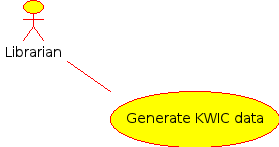
\includegraphics[scale=1]{use_case.png}}
             \caption{Simple use case diagram}
             \label{fig:class_diag}
        \end{center}
\end{figure}


\subsection{KWIC class diagram}
    \item[class diagram]    
     \begin{figure}[htb]
         \begin{center}
             \setlength\fboxsep{0pt}
             \fbox{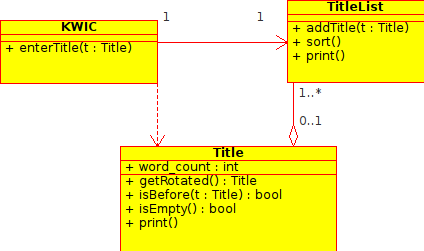
\includegraphics[scale=1]{class_diagram.png}}
             \caption{Class diagram}
             \label{fig:class_diag}
        \end{center}
\end{figure}


\subsection{KWIC sequance diagram}

    \item[class diagram]    
     \begin{figure}[htb]
         \begin{center}
             \setlength\fboxsep{0pt}
             \fbox{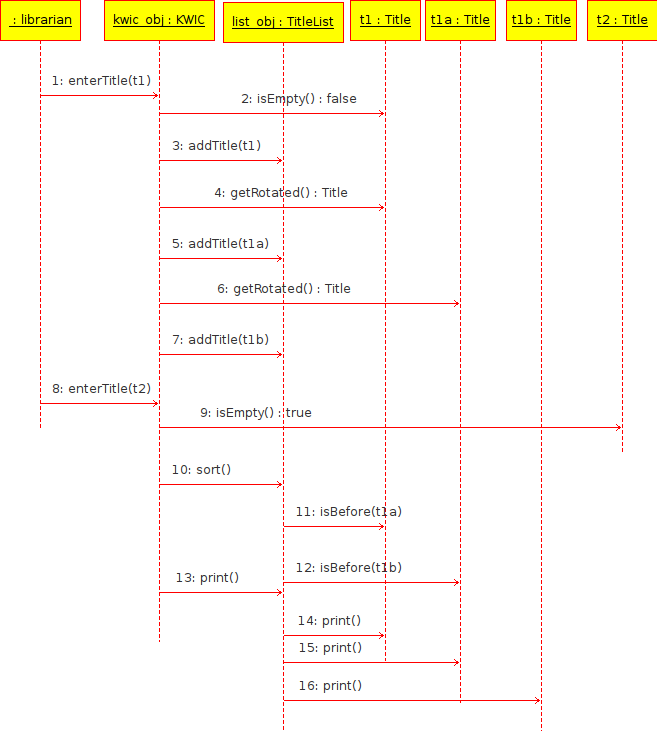
\includegraphics[scale=0.9]{sequence_diagram.png}}
             \caption{Sequence diagram}
             \label{fig:class_diag}
        \end{center}
\end{figure}

\end{description}


\end{document}
